\section{Shortcomings of \textit{SBM}}
\label{sec:Shortcomings}

Even though the \textit{SBM} methodology is a promising approach, it does not come without some serious shortcomings. These problems lie in three main characteristics of the method, namely:
\begin{itemize}
\item Construction of the predicate three
\item Search algorithm for similar predicates
\item The similarity evaluation function
\end{itemize}
In this section we demonstrate all these deficiencies with solid examples.

\subsection{Inclusion of Credibilities in Similarity Evaluation Function}
\label{cred}

The first defect of the \textit{SBM}approach comes with the way it utilizes the credibility values of the fuzzy rules in the similarity evaluation function for the predicates. The way that \textit{SBM} adopts proves to be problematic when the branching factor is small.  Since it's directly summed with the values of similarity pairs in the numerator of the equation, when the cardinality \textit{n} is small, the values of credibilities simply overshadow of similarity pairs.

\begin{ex}
The following simple example displays one such scenario:

\begin{center}
\begin{tabular}{l l}
$good\_basketball\_player:$  & $(Player)$\\

$bad\_basketball\_player:$ &  $(Player)$\\

$good\_technique:$ &  $(Player)$\\

$egoism:$ &  $(Player)$\\

\end{tabular}
\end{center}
\begin{tabular}{l l l}
$good\_basketball\_player(X)$ & $\stackrel{0.95,.}{\longleftarrow} prod$ & $good\_technique(X)$.\\

$bad\_basketball\_player(X)$ & $\stackrel{0.9,.}{\longleftarrow} prod$ & $egoism(X)$ .\\

\end{tabular}
\[Sim(good\_technique, egoism) = 0.1\]

\end{ex}

There is no need for expansion in this case for the predicate trees as they're structurally equivalent. The built trees are depicted in figure 1.14.
%[ref] \ref{basketJust}: 



\begin{figure}[h!] \label{basketJust}
\begin{center}
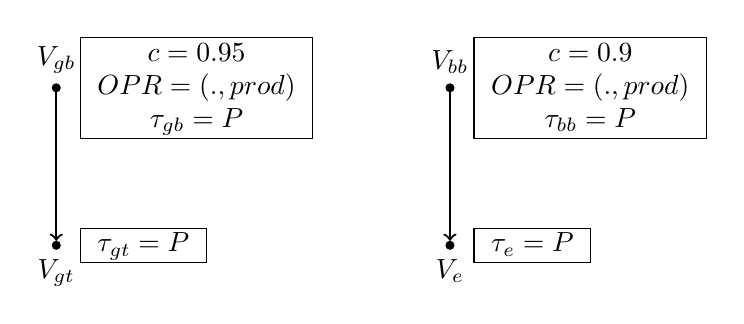
\begin{tikzpicture}[yscale=-1,
place/.style={circle,draw=black, fill=black, inner sep=0pt, 
              minimum size=1mm}]

\node[place] (1st) at (0, 0) [label=above: $V_{gb}$,
                              label=right: {
             \begin{tabular}{|c|}
               \hline
               $c=0.95$ \\
               $OPR=(.,prod)$ \\
               $\tau_{gb}=P$ \\
               \hline
             \end{tabular} }] {};

\node[place] (2nd) at (0, 2) [label=below:  $V_{gt}$,
                                label=right: {
             \begin{tabular}{|c|}
               \hline
               $\tau_{gt}=P$\\
               %\textit{atmic mark} $0$ \\
               \hline
             \end{tabular} }
] {};
        
	\draw[->, thick] (1st) -- (2nd);

\begin{scope}[xshift=5cm]
 \node[place] (1st) at (0, 0) [label=above: $V_{bb}$,
                              label=right: {
             \begin{tabular}{|c|}
               \hline
               $c=0.9$ \\
               $OPR=(.,prod)$ \\
               $\tau_{bb}=P$ \\
               \hline
             \end{tabular} }] {};

\node[place] (2nd) at (0, 2) [label=below:  $V_{e}$,
                                label=right: {
             \begin{tabular}{|c|}
               \hline
               $\tau_{e}=P$\\
              % \textit{atomic mark} $0$\\
               \hline
             \end{tabular} }
] {};
        
	\draw[->, thick] (1st) -- (2nd);
\end{scope}

\end{tikzpicture}
\end{center}
\caption{Predicate trees for \textit{good\_basketball\_player} and \textit{bad\_basketball\_player}}
\label{fig:ExpansionTrHtf}   
\end{figure}




By inspecting the example, one should \textbf{not} expect the predicates \textit{good\_basketball\_player} and \textit{bad\_basketball\_player} to be similar at all. We shall pursue via performing steps of \textit{SBM} in order to see if the expectation is consistent with the methodology's calculation.

$M_{s}$ = \{ (good\_technique, egoism)\}, $c^a$ = 0.95, $c^b$ = 0.9,   \textit{n} = 1.     

\begin{equation}\label{eq:sbmE1}
\begin{split}
M_v &=\frac{\sum_{i=1}^{1} v_i+1-\lvert c^a-c^b\rvert}{n+1}\\
&=\frac{0.1 +1-\lvert 0.95 - 0.9\rvert}{1+1}\\
&= \frac{1.05}{2}\\
&\cong{\textbf{0.53}}
 \end{split} 
\end{equation}

So on contrary to what was expected, \textit{SBM} calculates \textit{good\_basketball\_player} and \linebreak \textit{bad\_basketball\_player} to be somewhat similar. As mentioned earlier, this problem is caused by the fact that the equation does not integrate the credibility values in a proper way, thus in some cases (such as the branching factor is low) the emphasize is so high that it dominates the similarity values between the subpredicates. 

\subsection{Convergence to Identity Predicate}
\label{conv}
Earlier it was stated that in order to compare two predicates, \textit{SBM} needs them to have the same tree structure. And in order to accomplish this when they are not equal, the missing branches and leaves of the smaller tree are filled with identity predicates. Moreover a default similarity value is defined between an arbitrary predicate and the identity predicate. 

Unfortunately this introduces a couple of problems concerning the precision of the algorithm's final result. Similar to the effect that credibility values had in the previous section, this time we may have such an overwhelming impact from the default similarity values that is defined between the identity predicate and an arbitrary predicate.  One will especially encounter this kind of scenarios when one tree has high branching factor compared to the other one.


\begin{ex}
We see an example of such a case in the following program:
\begin{center}
\begin{tabular}{l l}
$classy\_restaurant:$  & $(Restaurant)$\\

$good\_restaurant:$  & $(Restaurant)$\\

$well\_trained\_waiters:$  & $(Restaurant)$\\

$expensive\_inventory:$  & $(Restaurant)$\\

$has\_good\_service:$  & $(Restaurant)$\\

$has\_healthy\_food:$  & $(Restaurant)$\\

$has\_tasty\_food:$  & $(Restaurant)$\\

$has\_nice\_surroundings:$  & $(Restaurant)$\\

$has\_high\_reputation:$  & $(Restaurant)$\\

\end{tabular}
\end{center}
\begin{tabular}{l l l}
$classy\_restaurant(X)$ & $\stackrel{1.0,.}{\longleftarrow} prod$ & $well\_trained\_waiters(X), expensive\_inventory(X).$\\

$good\_restaurant(X)$ & $\stackrel{0.95,.}{\longleftarrow} prod$ & $has\_healthy\_food(X), has\_good\_service(X),$\\ 
%$has\_nice\_surroundings(X), $ & $has\_nice\_surroundings(X),$ $has\_nice\_surroundings(X), $\\
$ $ & $$ & $has\_nice\_surroundings(X), has\_high\_reputation(X),$\\
$ $ & $$ & $has\_tasty\_food(X).$\\

\end{tabular}
\[Sim(well\_trained\_waiters, has\_good\_service) = 0.9\]
\[Sim(expensive\_inventory, has\_nice\_surroundings) = 0.8\]
\end{ex}

Regarding to the program we should expect the predicates \textit{classy\_restaurant} and \linebreak[4] \textit{good\_restaurant} to have a high similarity degree.

Once again we should start via constructing the predicate trees for  \textit{BMS}. As the two trees are not structurally equal, the smaller tree, the predicate tree of \textit{classy\_restaurant} must be expanded.



 \begin{figure}[h!]
\begin{center}
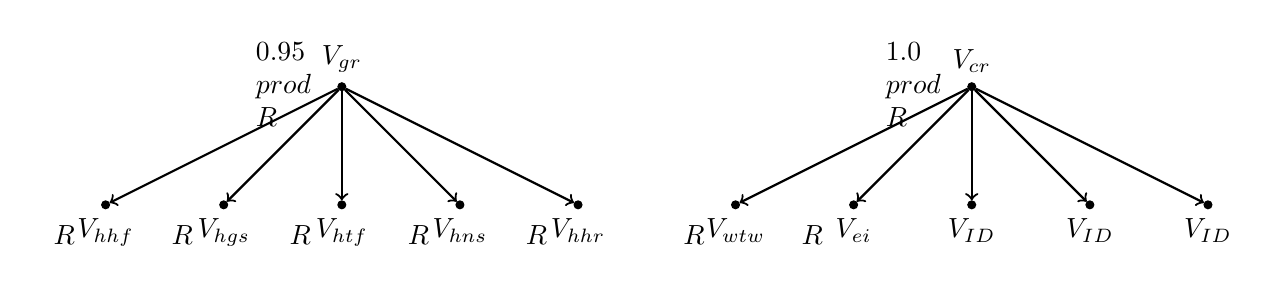
\begin{tikzpicture}[yscale=-1,
place/.style={circle,draw=black, fill=black, inner sep=0pt, 
              minimum size=1mm}]

  \node[place] (1st) at (3, 0) [label=above: $V_{gr}$,
                                  label=left: 
     \begin{tabular}{l}
        $0.95$\\
        $prod$\\
        $R$\\  
     \end{tabular}
] {};
  \node[place] (2nd) at (0, 1.5) [label=below: $V_{hhf}$,
                                  label=left:
     \begin{tabular}{l}
        $$\\
        $$\\
        $R$\\  
     \end{tabular}
]{};
  \node[place] (3rd) at (1.5, 1.5)  [label=below: $V_{hgs}$,
                                  label=left:
     \begin{tabular}{l}
        $$\\
        $$\\
        $R$\\  
     \end{tabular}	] {}; 
  \node[place] (4th) at (3, 1.5)   [label=below: $V_{htf}$,
                                  label=left:
     \begin{tabular}{l}
        $$\\
        $$\\
        $R$\\  
     \end{tabular}
             ] {}; 
             
 \node[place] (5th) at (4.5, 1.5) [label=below: $V_{hns}$,
                                  label=left:
     \begin{tabular}{l}
        $$\\
        $$\\
        $R$\\  
     \end{tabular}
             ] {}; 
             
             
   \node[place] (6th) at (6, 1.5)  [label=below: $V_{hhr}$,
                                  label=left:
     \begin{tabular}{l}
        $$\\
        $$\\
        $R$\\  
     \end{tabular}
             ] {};     

  %\node (dots) at (2,1.5) {$\cdots$};
	
  \draw[->, thick] (1st) -- (2nd);
  \draw[->, thick] (1st) -- (3rd);
  \draw[->, thick] (1st) -- (4th);
  \draw[->, thick] (1st) -- (5th);
  \draw[->, thick] (1st) -- (6th);

\begin{scope}[xshift=8cm]
  \node[place] (1st) at (3, 0) [label=above: $V_{cr}$,
                                  label=left: 
     \begin{tabular}{l}
        $1.0$\\
        $prod$\\
        $R$\\  
     \end{tabular}
] {};

  \node[place] (2nd) at (0, 1.5) [label=below: $V_{wtw}$,
                                  label=left:
     \begin{tabular}{l}
        $$\\
        $$\\
        $R$\\  
     \end{tabular}
]{};
  \node[place] (3rd) at (1.5, 1.5)  [label=below: $V_{ei}$,
                                  label=left:
     \begin{tabular}{l}
        $$\\
        $$\\
        $R$\\  
     \end{tabular}	] {}; 
  \node[place] (4th) at (3, 1.5)   [label=below: $V_{ID}$,
                                  label=left:
     \begin{tabular}{l}
        $$\\
        $$\\
       % $R$\\  
     \end{tabular}
             ] {}; 
             
 \node[place] (5th) at (4.5, 1.5) [label=below: $V_{ID}$,
                                  label=left:
     \begin{tabular}{l}
        $$\\
        $$\\
      %  $R$\\  
     \end{tabular}
             ] {}; 
             
             
   \node[place] (6th) at (6, 1.5)  [label=below: $V_{ID}$,
                                  label=left:
     \begin{tabular}{l}
        $$\\
        $$\\
   %     $R$\\  
     \end{tabular}
             ] {};     

%  \node (dots) at (1,1.5) {$\cdots$};
	
\draw[->, thick] (1st) -- (2nd);
  \draw[->, thick] (1st) -- (3rd);
  \draw[->, thick] (1st) -- (4th);
  \draw[->, thick] (1st) -- (5th);
  \draw[->, thick] (1st) -- (6th);
\end{scope}

);
\end{tikzpicture}
\end{center}
\caption{Predicate trees in expanded form for \textit{SBM}}
\label{fig:res1}
\end{figure}

%\newpage
There is only one level of expansion. Since at every level the $M_{s}$ that leads to the highest degree of similarity is chosen, the corresponding decision set will be: $M_{ds}$ = \textit{\{ (well\_trained\_waiters, has\_good\_service), (expensive\_inventory, has\_nice\_surroundings), (ID, has\_healthy\_food), (ID, has\_tasty\_food), (ID, has\_high\_reputation)\}}

One thing that we should pay attention to is that, since in this example, \textit{BMS} needed the introduction of the \textit{Identity Predicate}, a default similarity value  between an arbitrary predicate and the identity predicate should also be defined. Assume \textit{Sim(ID, p) = 0.3} for any arbitrary predicate.  

The rest of the variable values are as follows:

$c^a$ = 0.95, $c^b$ = 1,   \textit{n} = 5.     

\begin{equation}\label{eq:sbmE2}
\begin{split}
M_v &=\frac{\sum_{i=1}^{5} v_i+1-\lvert c^a-c^b\rvert}{n+1}\\
&=\frac{2.9 +1-\lvert 0.95 - 1\rvert}{5+1}\\
%&= \frac{1.05}{2}\\
&\cong{\textbf{0.55}}
 \end{split} 
\end{equation}

In this case the algorithm was not able to successfully evaluate and conclude that the predicates are actually closely related. This distortion was caused because of the relatively big branching factor difference and the identity predicates introduced for the missing one. As one can see, in \textit{SBM} as \textit{\textbf{the missing number of nodes in one tree increases,  the similarity degree calculated by the algorithm converges to the default values}} that is defined between an arbitrary predicate and the identity predicate.

One should suspect that an  algorithm which does not introduce any such external knowledge, and just use the original information of the knowledge base, might prevent having such shortcomings.













\subsection{Wrong Filtering}
\label{filt}

In her work Lu makes the following assumption \cite{Lu}:

\textit{...However, practically, the number of corresponding trees for certain predicate will not achieve the exponential, since the rules will be defined more reasonable, rather than the given example.} 

%I do not agree with this premise as I believe a computer scientist must always develop algorithms which would correctly terminate for any given input setting.

This premise proves to be dangerous as making assumptions on the input setting may cause algorithms to contain flaws.

There is one other faulty behavior of \textit{SBM} which is caused from this relaxed assumption of the the knowledge bases. After every level of expansion, \textit{SBM} checks every predicate pair between the two trees with respect to their resulting similarity degree. Before the next level of expansion is pursued, a filtering is done on the tree by selecting the best pair combination on the level. The problem with this approach is that the information on a prior level is incomplete, and thus wrong steps can be taken when filtering that will cause the loss of crucial information for the main focus, \textit{i.e}. comparing the similarity values of the main predicates.  

Since the previous thesis work does not include any examples with predicate trees deeper then just one level, we try to demonstrate the problem with the following example:




\begin{ex}
The program consists of following type declarations and rules:

\begin{center}
\begin{tabular}{l l}

$modern\_city:$  & $(City)$\\

$livable\_city:$  & $(City)$\\

$life\_expectancy:$  & $(Society)$\\

$birth\_rate:$  & $(Society)$\\

$social\_welfare:$  & $(Society)$\\

$\#of\_schools$  & $(Society)$\\

$quality\_of\_academic\_staff$  & $(Society)$\\

$\#of\_teachers$  & $(Society)$\\

$compulsory\_schooling\_length$  & $(Society)$\\

$educated\_society:$  & $(Society)$\\

$\#of\_healthy\_individuals$  & $(Society)$\\

$literacy\_rate:$  & $(Society)$\\

$high\_population:$  & $(Society)$\\



\end{tabular}
\end{center}
\begin{tabular}{l l l}
$livable\_city(X)$ & $\stackrel{0.8,.}{\longleftarrow} prod$ & $literacy\_rate(X), \#of\_healthy\_individuals(X).$\\

$literacy\_rate(X)$ & $\stackrel{1.0,.}{\longleftarrow} prod$ & $compulsory\_schooling\_length(X), \#of\_teachers(X).$\\

$modern\_city(X)$ & $\stackrel{0.7,.}{\longleftarrow} prod$ & $educated\_society(X), high\_population(X),$\\ $$ & $$ & $social\_welfare(X).$\\ 
%$has\_nice\_surroundings(X), $ & $has\_nice\_surroundings(X),$ $has\_nice\_surroundings(X), $\\
%$ $ & $$ & $has\_nice\_surroundings(X), has\_high\_reputation(X).$\\
$educated\_society(X)$ & $\stackrel{1.0,.}{\longleftarrow} prod$ & $\#of\_schools(X), quality\_of\_academic\_staff(X).$\\ 
$high\_population(X)$ & $\stackrel{1,0,.}{\longleftarrow} prod$ & $birth\_rate(X), life\_expectancy(X).$\\ 


\end{tabular}
\[Sim(compulsory\_schooling\_length, \#of\_schools) = 0.9\]
\[Sim(\#of\_teachers, quality\_of\_academic\_staff) = 0.85\]
\[Sim(literacy\_rate, social\_welfare) = 0.4\]
\[Sim(\#of\_healthy\_individuals, life\_expectancy) = 0.7\]
\end{ex}


Focus of interest is evaluating the similarity degree of \textit{livable\_city} and \textit{modern\_city}. Let's start calculating this value via our algorithm.



\begin{figure}[h!]
\begin{center}
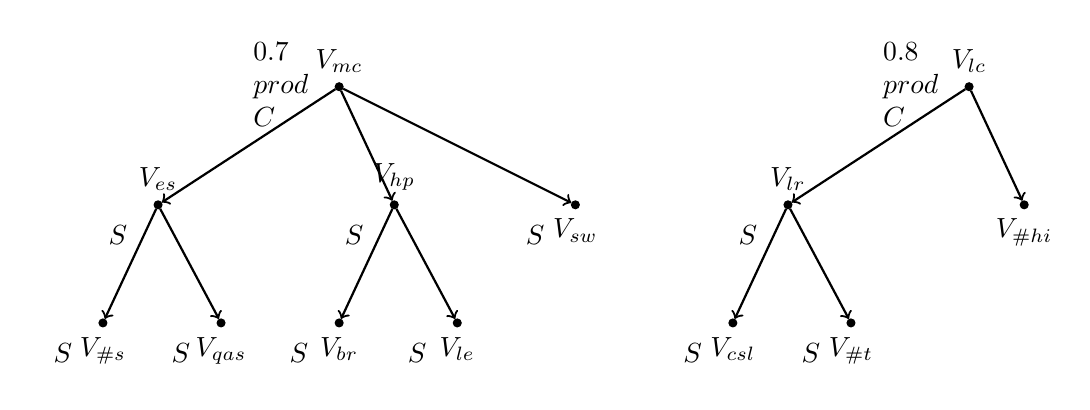
\begin{tikzpicture}[yscale=-1,
place/.style={circle,draw=black, fill=black, inner sep=0pt, 
              minimum size=1mm}]

  \node[place] (1st) at (3, 0) [label=above: $V_{mc}$,
                                  label=left: 
     \begin{tabular}{l}
        $0.7$\\
        $prod$\\
        $C$\\  
     \end{tabular}
] {};
  \node[place] (2nd) at (0.7, 1.5) [label=above: $V_{es}$,
                                  label=left:
     \begin{tabular}{l}
        $$\\
        $$\\
        $S$\\  
     \end{tabular}
]{};
  \node[place] (3rd) at (3.7, 1.5)  [label=above: $V_{hp}$,
                                  label=left:
     \begin{tabular}{l}
        $$\\
        $$\\
        $S$\\  
     \end{tabular}	] {}; 
  \node[place] (4th) at (6, 1.5)   [label=below: $V_{sw}$,
                                  label=left:
     \begin{tabular}{l}
        $$\\
        $$\\
        $S$\\  
     \end{tabular}
             ] {}; 
             
             
             
             
             
               \node[place] (5th) at (0, 3) [label=below: $V_{\#s}$,
                                  label=left:
     \begin{tabular}{l}
        $$\\
        $$\\
        $S$\\  
     \end{tabular}
]{};  

\node[place] (6th) at (1.5, 3) [label=below: $V_{qas}$,
                                  label=left:
     \begin{tabular}{l}
        $$\\
        $$\\
        $S$\\  
     \end{tabular}
]{};
  
  
                 \node[place] (7th) at (3, 3) [label=below: $V_{br}$,
                                  label=left:
     \begin{tabular}{l}
        $$\\
        $$\\
        $S$\\  
     \end{tabular}
]{};  

\node[place] (8th) at (4.5, 3) [label=below: $V_{le}$,
                                  label=left:
     \begin{tabular}{l}
        $$\\
        $$\\
        $S$\\  
     \end{tabular}
]{};
  
  

  
  
  
  
  
  %\node (dots) at (2,1.5) {$\cdots$};
	
  \draw[->, thick] (1st) -- (2nd);
  \draw[->, thick] (1st) -- (3rd);
  \draw[->, thick] (1st) -- (4th);
    \draw[->, thick] (2nd) -- (5th);
      \draw[->, thick] (2nd) -- (6th);
          \draw[->, thick] (3rd) -- (7th);
      \draw[->, thick] (3rd) -- (8th);

\begin{scope}[xshift=8cm]
    \node[place] (1st) at (3, 0) [label=above: $V_{lc}$,
                                  label=left: 
     \begin{tabular}{l}
        $0.8$\\
        $prod$\\
        $C$\\  
     \end{tabular}
] {};
  \node[place] (2nd) at (0.7, 1.5) [label=above: $V_{lr}$,
                                  label=left:
     \begin{tabular}{l}
        $$\\
        $$\\
        $S$\\  
     \end{tabular}
]{};
  \node[place] (3rd) at (3.7, 1.5)  [label=below: $V_{\#hi}$,
                                  label=left:
     \begin{tabular}{l}
        $$\\
        $$\\
       % $S$\\  
     \end{tabular}	] {}; 

             
             
             
             
             
               \node[place] (5th) at (0, 3) [label=below: $V_{csl}$,
                                  label=left:
     \begin{tabular}{l}
        $$\\
        $$\\
        $S$\\  
     \end{tabular}
]{};  

\node[place] (6th) at (1.5, 3) [label=below: $V_{\#t}$,
                                  label=left:
     \begin{tabular}{l}
        $$\\
        $$\\
        $S$\\  
     \end{tabular}
]{};
  
    
  
  



  \draw[->, thick] (1st) -- (2nd);
  \draw[->, thick] (1st) -- (3rd);
    \draw[->, thick] (2nd) -- (5th);
      \draw[->, thick] (2nd) -- (6th);






\end{scope}

);
\end{tikzpicture}
\end{center}
\caption{Predicate trees of \textit{livable\_city} and \textit{modern\_city} in original form}
\label{fig:res1}
\end{figure}


\newpage
By know we know that as trees are do not share the same tree strcuture, \textit{SBM} needs reconstructed versions of the tree before the evaluation algorithm can work. 



% --------------------------------------------------------------------------------------------

%\newpage

 \begin{figure}[h!]
\begin{center}
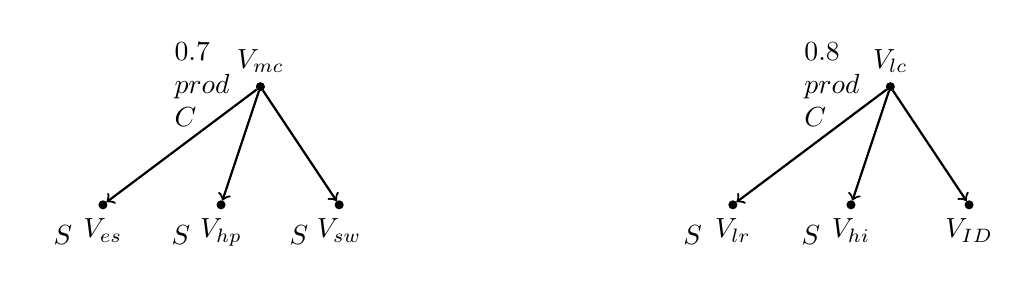
\begin{tikzpicture}[yscale=-1,
place/.style={circle,draw=black, fill=black, inner sep=0pt, 
              minimum size=1mm}]

  \node[place] (1st) at (2, 0) [label=above: $V_{mc}$,
                                  label=left: 
     \begin{tabular}{l}
        $0.7$\\
        $prod$\\
        $C$\\  
     \end{tabular}
] {};
  \node[place] (2nd) at (0, 1.5) [label=below: $V_{es}$,
                                  label=left:
     \begin{tabular}{l}
        $$\\
        $$\\
        $S$\\  
     \end{tabular}
]{};
  \node[place] (3rd) at (1.5, 1.5)  [label=below: $V_{hp}$,
                                  label=left:
     \begin{tabular}{l}
        $$\\
        $$\\
        $S$\\  
     \end{tabular}	] {}; 
  \node[place] (4th) at (3, 1.5)   [label=below: $V_{sw}$,
                                  label=left:
     \begin{tabular}{l}
        $$\\
        $$\\
        $S$\\  
     \end{tabular}
             ] {}; 
  
  %\node (dots) at (2,1.5) {$\cdots$};
	
  \draw[->, thick] (1st) -- (2nd);
  \draw[->, thick] (1st) -- (3rd);
  \draw[->, thick] (1st) -- (4th);

\begin{scope}[xshift=8cm]
  \node[place] (1st) at (2, 0) [label=above: $V_{lc}$,
                                  label=left: 
     \begin{tabular}{l}
        $0.8$\\
        $prod$\\
        $C$\\  
     \end{tabular}
] {};

  \node[place] (2nd) at (0, 1.5) [label=below: $V_{lr}$,
                                  label=left:
     \begin{tabular}{l}
        $$\\
        $$\\
        $S$\\  
     \end{tabular}
]{};
  \node[place] (3rd) at (1.5, 1.5)  [label=below: $V_{hi}$,
                                  label=left:
     \begin{tabular}{l}
        $$\\
        $$\\
        $S$\\  
     \end{tabular}	] {}; 
  \node[place] (4th) at (3, 1.5)   [label=below: $V_{ID}$,
                                  label=left:
     \begin{tabular}{l}
        $$\\
        $$\\
       % $R$\\  
     \end{tabular}
             ] {}; 

%  \node (dots) at (1,1.5) {$\cdots$};
	
\draw[->, thick] (1st) -- (2nd);
  \draw[->, thick] (1st) -- (3rd);
  \draw[->, thick] (1st) -- (4th);

\end{scope}

);
\end{tikzpicture}
\end{center}
\caption{Predicate trees after one level of expansion in \textit{SBM}}
\label{fig:res1}
\end{figure}

After the first expansion is done, again an identity predicate is introduced for the missing leaf node in the predicate tree with the root \textit{livable\_city}. The problem arise in this step. As we have discussed before, \textit{SBM} makes a filtering of the node-pairs before the next expansion, with respect to the similarity proximities of the pairs in this level. And once again as we have mentioned, this as most of the information hidden in the lower levels is not apparent to the algorithm yet, filtering can cause neglecting some important paths of the tree.

For instance at this point, between the node pairs, only a similarity relation between the predicates \textit{literacy\_rate} and \textit{social\_welfare} is defined. The algorithm continues expanding, via selecting the \textit{middle set} with the highest similarity value at the current value as the \textit{decision middle set}. So in this example, at the first level \textit{$M_{ds}$} = \{ (\textit{$V_{sw }$} , \textit{$V_{lr}$} ), (\textit{$V_{hp }$} , \textit{$V_{ID}$} ) \}  or \textit{$M_{ds}$} = \{ (\textit{$V_{sw }$} , \textit{$V_{lr}$} ), (\textit{$V_{es }$} , \textit{$V_{ID}$} ) \}  as they prove to be the best of the \textit{$M_{s}$} sets.


% --------------------------------------------------------------------------------------------




\begin{figure}[h!]
\begin{center}
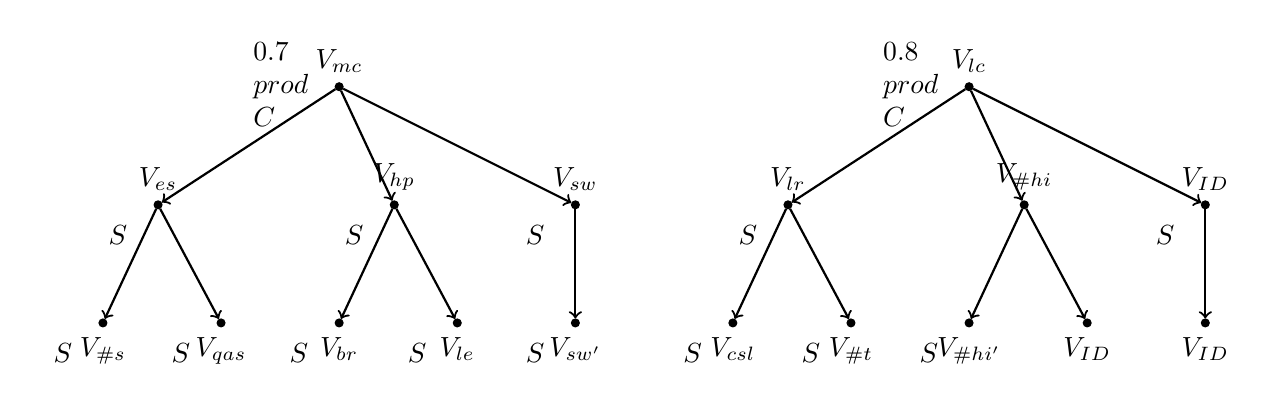
\begin{tikzpicture}[yscale=-1,
place/.style={circle,draw=black, fill=black, inner sep=0pt, 
              minimum size=1mm}]

  \node[place] (1st) at (3, 0) [label=above: $V_{mc}$,
                                  label=left: 
     \begin{tabular}{l}
        $0.7$\\
        $prod$\\
        $C$\\  
     \end{tabular}
] {};
  \node[place] (2nd) at (0.7, 1.5) [label=above: $V_{es}$,
                                  label=left:
     \begin{tabular}{l}
        $$\\
        $$\\
        $S$\\  
     \end{tabular}
]{};
  \node[place] (3rd) at (3.7, 1.5)  [label=above: $V_{hp}$,
                                  label=left:
     \begin{tabular}{l}
        $$\\
        $$\\
        $S$\\  
     \end{tabular}	] {}; 
  \node[place] (4th) at (6, 1.5)   [label=above: $V_{sw}$,
                                  label=left:
     \begin{tabular}{l}
        $$\\
        $$\\
        $S$\\  
     \end{tabular}
             ] {}; 
             
             
             
             
             
               \node[place] (5th) at (0, 3) [label=below: $V_{\#s}$,
                                  label=left:
     \begin{tabular}{l}
        $$\\
        $$\\
        $S$\\  
     \end{tabular}
]{};  

\node[place] (6th) at (1.5, 3) [label=below: $V_{qas}$,
                                  label=left:
     \begin{tabular}{l}
        $$\\
        $$\\
        $S$\\  
     \end{tabular}
]{};
  
  
                 \node[place] (7th) at (3, 3) [label=below: $V_{br}$,
                                  label=left:
     \begin{tabular}{l}
        $$\\
        $$\\
        $S$\\  
     \end{tabular}
]{};  

\node[place] (8th) at (4.5, 3) [label=below: $V_{le}$,
                                  label=left:
     \begin{tabular}{l}
        $$\\
        $$\\
        $S$\\  
     \end{tabular}
]{};
  
  
  
                 \node[place] (9th) at (6, 3) [label=below: $V_{sw'}$,
                                  label=left:
     \begin{tabular}{l}
        $$\\
        $$\\
        $S$\\  
     \end{tabular}
]{};  


  
  
  
  
  
  %\node (dots) at (2,1.5) {$\cdots$};
	
  \draw[->, thick] (1st) -- (2nd);
  \draw[->, thick] (1st) -- (3rd);
  \draw[->, thick] (1st) -- (4th);
    \draw[->, thick] (2nd) -- (5th);
      \draw[->, thick] (2nd) -- (6th);
          \draw[->, thick] (3rd) -- (7th);
      \draw[->, thick] (3rd) -- (8th);
          \draw[->, thick] (4th) -- (9th);

\begin{scope}[xshift=8cm]
    \node[place] (1st) at (3, 0) [label=above: $V_{lc}$,
                                  label=left: 
     \begin{tabular}{l}
        $0.8$\\
        $prod$\\
        $C$\\  
     \end{tabular}
] {};
  \node[place] (2nd) at (0.7, 1.5) [label=above: $V_{lr}$,
                                  label=left:
     \begin{tabular}{l}
        $$\\
        $$\\
        $S$\\  
     \end{tabular}
]{};
  \node[place] (3rd) at (3.7, 1.5)  [label=above: $V_{\#hi}$,
                                  label=left:
     \begin{tabular}{l}
        $$\\
        $$\\
       % $S$\\  
     \end{tabular}	] {}; 
  \node[place] (4th) at (6, 1.5)   [label=above: $V_{ID}$,
                                  label=left:
     \begin{tabular}{l}
        $$\\
        $$\\
        $S$\\  
     \end{tabular}
             ] {}; 
             
             
             
             
             
               \node[place] (5th) at (0, 3) [label=below: $V_{csl}$,
                                  label=left:
     \begin{tabular}{l}
        $$\\
        $$\\
        $S$\\  
     \end{tabular}
]{};  

\node[place] (6th) at (1.5, 3) [label=below: $V_{\#t}$,
                                  label=left:
     \begin{tabular}{l}
        $$\\
        $$\\
        $S$\\  
     \end{tabular}
]{};
  
  
                 \node[place] (7th) at (3, 3) [label=below: $V_{\#hi'}$,
                                  label=left:
     \begin{tabular}{l}
        $$\\
        $$\\
        $S$\\  
     \end{tabular}
]{};  

\node[place] (8th) at (4.5, 3) [label=below: $V_{ID}$,
                                  label=left:
     \begin{tabular}{l}
        $$\\
        $$\\
       % $S$\\  
     \end{tabular}
]{};
  
  
  
                 \node[place] (9th) at (6, 3) [label=below: $V_{ID}$,
                                  label=left:
     \begin{tabular}{l}
        $$\\
        $$\\
    %    $S$\\  
     \end{tabular}
]{};  


  \draw[->, thick] (1st) -- (2nd);
  \draw[->, thick] (1st) -- (3rd);
  \draw[->, thick] (1st) -- (4th);
    \draw[->, thick] (2nd) -- (5th);
      \draw[->, thick] (2nd) -- (6th);
          \draw[->, thick] (3rd) -- (7th);
      \draw[->, thick] (3rd) -- (8th);
          \draw[->, thick] (4th) -- (9th);





\end{scope}

);
\end{tikzpicture}
\end{center}
\caption{Predicate trees after two levels of expansion in \textit{SBM}}
\label{fig:res1}
\end{figure}




\

However this local optimization approach eliminates other fruitful pair combinations such as \textit{social\_welfare} and \textit{educated\_society}. In \textit{Figure 6} this pair corresponds to the left subtrees of the main predicate trees. These prove to be the most similar subconcepts of the two as there are two leaf node pairs for which the similarity relation is defined via values \textit{0.9} and \textit{0.85}. 

All in all, wrong choice for filtering causes comparing wrong pairs of subpredicates in the end and thus a distorted final similarity degree between the predicates of interest.


% --------------------------------------------------------------------------------------------



\subsection{Shared Similarity Concepts}
\label{sharedSim}

Another shortcoming of the \textit{SBM} approach is that since it does a one to one mapping between the subconcepts of the main predicates,  it can not utilize the information given in the knowledge base completely where a particular concept is included in more then one similarity relations.

\begin{ex}
Let us observe the following simple program:
\begin{center}
\begin{tabular}{l l}
$touristic\_place:$  & $(Land)$\\

$nice\_destinationt:$  & $(Land)$\\

$cultural\_venues:$  & $(Sight)$\\

$natural\_wonders:$  & $(Sight)$\\

$many\_sights:$  & $(Sight)$\\

$good\_weather:$  & $(Temperature)$\\

\end{tabular}
\end{center}
\begin{tabular}{l l l}
$touristic\_place(X)$ & $\stackrel{1.0,.}{\longleftarrow} prod$ & $cultural\_venues(X), natural\_wonders(X).$\\

$nice\_destination(X)$ & $\stackrel{1.0,.}{\longleftarrow} prod$ & $good\_weather(X), many\_sights(X).$\\


\end{tabular}
\[Sim(cultural\_venues, many\_sights) = 0.7\]
\[Sim(natural\_wonders, many\_sights) = 0.7\]
\end{ex}

%\newpage
In the evaluation step, since both of the similarity degrees are equal the algorithm will conclude that there are two optimal \textit{$M_{ds}$}. It will either conclude \textit{$M_{ds}$} \linebreak = \{ (\textit{$V_{cv }$} , \textit{$V_{ms}$} )  \} and the pair (\textit{$V_{nw }$} , \textit{$V_{gw}$} ) to be incomparable, or the counter case where \textit{$M_{ds}$} = \{ (\textit{$V_{nw }$} , \textit{$V_{ms}$} )  \} and the pair (\textit{$V_{cv }$} , \textit{$V_{gw}$} ) to be incomparable. In both cases the algorithm is bound to miss on the similarity relations and thus the evaluation algorithm can not utilize that data.
\newpage
In the case for which the proximity of similarity of the relations were different, that time the algorithm would simply neglect the smaller one. Thus again half of the information in the knowledge base would be lost without chance of recovery.

%\begin{comment}

\begin{figure}[t!]
\begin{center}
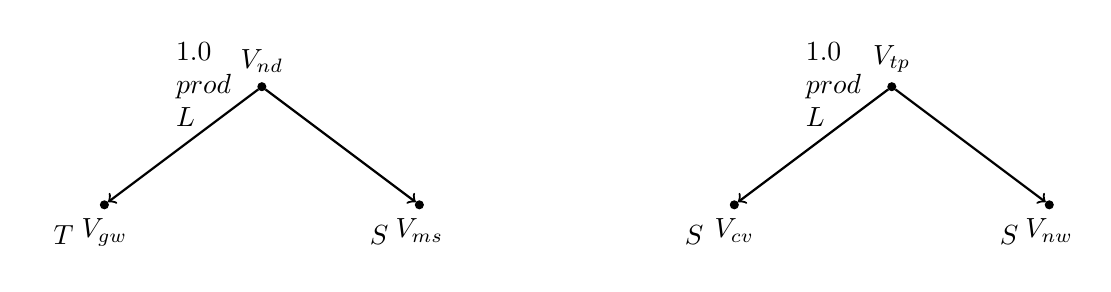
\begin{tikzpicture}[yscale=-1,
place/.style={circle,draw=black, fill=black, inner sep=0pt, 
              minimum size=1mm}]

  \node[place] (1st) at (2, 0) [label=above: $V_{nd}$,
                                  label=left: 
     \begin{tabular}{l}
        $1.0$\\
        $prod$\\
        $L$\\  
     \end{tabular}
] {};
  \node[place] (2nd) at (0, 1.5) [label=below: $V_{gw}$,
                                  label=left:
     \begin{tabular}{l}
        $$\\
        $$\\
        $T$\\  
     \end{tabular}
]{};
  \node[place] (3rd) at (4, 1.5)  [label=below: $V_{ms}$,
                                  label=left:
     \begin{tabular}{l}
        $$\\
        $$\\
        $S$\\  
     \end{tabular}	] {}; 
 

  %\node (dots) at (2,1.5) {$\cdots$};
	
  \draw[->, thick] (1st) -- (2nd);
  \draw[->, thick] (1st) -- (3rd);

\begin{scope}[xshift=8cm]
  \node[place] (1st) at (2, 0) [label=above: $V_{tp}$,
                                  label=left: 
     \begin{tabular}{l}
        $1.0$\\
        $prod$\\
        $L$\\  
     \end{tabular}
] {};

  \node[place] (2nd) at (0, 1.5) [label=below: $V_{cv}$,
                                  label=left:
     \begin{tabular}{l}
        $$\\
        $$\\
        $S$\\  
     \end{tabular}
]{};
  \node[place] (3rd) at (4, 1.5)  [label=below: $V_{nw}$,
                                  label=left:
     \begin{tabular}{l}
        $$\\
        $$\\
        $S$\\  
     \end{tabular}	] {}; 

             ] {};     

%  \node (dots) at (1,1.5) {$\cdots$};
	
\draw[->, thick] (1st) -- (2nd);
  \draw[->, thick] (1st) -- (3rd);
\end{scope}

);
\end{tikzpicture}
\end{center}
\caption{Predicate trees for \textit{nice\_destination} and \textit{touristic\_place}}
\label{fig:placeJust}
\end{figure}

%\end{comment}
